\graphicspath{{fig/missing/}%
              {fig/scoters/}}

\chapter{Missing data}
\label{cha:missing}

Collecting data of flocking events is a demanding process (see, for example,
\textcite{cavagna08a} and \textcite{lukeman10}). Along with the technical
challenges posed by data collection, flocking events are inherently
unpredictable, and so it is not possible to know when and where a flocking
event may occur next. In this way there can become a frustrating
``right-place-right-time'' component to data collection.

Typically, recording equipment is set up in a fixed location where the
scientist believes a flocking event may occur \parencite{lukeman10}. Stationary
recording equipment results in a fixed field of vision in which data may be
captured. Unfortunately, this stationary set-up can result in recording
incomplete flocking events. This may happen when flock members stray outside
the field of vision during a recording event. As the recording equipment is
fixed in location the field of vision cannot be adjusted to reinclude those who
move out-of-frame.

The flock members which move out of frame \emph{cannot} be ignored during
analysis: although we may not observe their movements, they may still be
influencing the behaviour of the flock, and so must be accounted for. A simple
but undesirable solution is presented by the temptation to discard \emph{every}
frame in which \emph{any} individual is out of view. This ``solution'' has the
potential to drastically reduce the amount of data available for analysis. As
capturing flocking events can be such an involved and time-consuming endeavour,
it seems remiss to discard observations and the information they contain.

In this chapter we will consider how we can handle flocking events which
contain missing observations. The movements of missing agents will not be
ignored, nor will data be discarded. Instead, we will work in a Bayesian framework
to adjust our posterior densities about model parameters to account for
unobserved behaviours. We will see that this can be achieved by integrating
over all the possible trajectories of missing agents. We show that
this approach gives more accurate results than the naive approach of discarding
data, before demonstrating the developed methodology on real observation.

\section{Types of missingness}
\label{sec:missing_types}

When we consider flocking events with missing observations, it is important to
consider at which point during the sequence a given agent went missing. This is
because how we account for the missingness will depend on at which point during
the sequence the agent went missing.

Although there are many different circumstances which can result in an agent
leaving our visual field, here we shall inspect the two cases which we consider
as the most likely to occur. These two cases arise when agents are out of frame
at the \emph{beginning} of a recording event, or when agents are out of frame
at the \emph{end} of a recording event.

We shall integrate over the possible missing observations using a
Metropolis--Hastings scheme. A proposal mechanism for generating paths missing
at the beginning of a sequence is outlined. Proposed paths can then be accepted
or rejected using results from \cref{cha:sim_studies}. We will then show that
we can generate paths missing at the end of a sequence by implementing a Gibbs
sampler (\cref{alg:gibbs}); sampling from our full conditional distributions to
realise a distribution of possible paths.

\subsection{Missing in the beginning of a sequence}
\label{ssec:beg_missing}

We say that data is missing at the beginning of a flocking event if the
observer began recording the sequence before all agents had entered the frame.
When we consider this case we assume that all the flock members do eventually
enter the visual field, and so the total number of individuals in the flock is
known.

We imitate this scenario by forward simulating the Vicsek model and imposing a
fixed field of vision on top of the resulting data. We chose to forward
simulate $25$ agents for $40$ time steps. At time $t=1$ agents were directed
and positioned randomly within a square-cell of side length $L=1$. Agents
experienced noise generated from a generalised Student's $t$-distribution with
$\nu=7$ degrees of freedom and scale $\sigma_Y=0.075$. Each individual
interacted with neighbours positioned within distance $r=0.5$, and moved with
speed $v=0.03$.

The resulting simulated data is illustrated in \cref{subfig:beg_data}. The
rectangle overlain in black represents a fixed field of vision: analogous to
the fixed visual field generated by recording equipment in the field. The
movements of agents outside this fixed area are classified as missing and are
represented by the red trajectories. Agents move from the positions denoted by
the green markers, to the positions represented by the red makers. The ID
number of each agent, $i$, is shown at the beginning and end of its trajectory.
It can be seen that some agents were \emph{outside} our visual field at the
beginning of the simulation. 

\cref{subfig:beg_missing} shows a schematic representing which data points of
our simulation were considered observed and which data points were classified
as missing. A blue gridpoint in location $(t, i)$ tells us that agent $i$
\emph{was observed} at time $t$. Conversely, a red maker at location $(t, i)$
indicates that agent $i$ \emph{was missing} at time $t$. From this schematic we
can see that a number of agents were classified as missing at time $t=1$: the
beginning of the simulation.

\begin{figure}[tbp]
  \captionsetup[subfigure]{oneside,
                           margin={0.7cm,0cm}}
  \begin{subfigure}[b]{0.5\textwidth}
    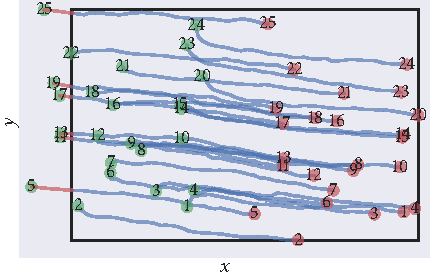
\includegraphics{beg/data.pdf}
    \caption{}
    \label{subfig:beg_data}
  \end{subfigure}%
  \begin{subfigure}[b]{0.5\textwidth}
    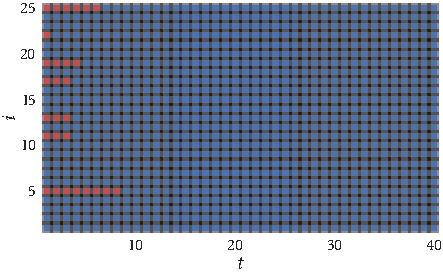
\includegraphics{beg/missing_array.pdf}
    \caption{}
    \label{subfig:beg_missing}
  \end{subfigure}
  \caption{Illustrating our forward simulation of the Vicsek model and the
    data considered missing. \subref{subfig:beg_data} Simulated trajectories.
    The rectangle overlain in black represents our imitation of a fixed
    field of vision: analogous to that of recording equipment used in the
    field. Agents travel from green marker to red marker, with their ID ($i$)
    shown at their start and end points. Data points outside of the rectangular
    region are classified as missing, and are shown by red trajectories.
    \subref{subfig:beg_missing} Summarising the missing and observed data
    points of our simulation. A blue gridpoint at location $(t, i)$ indicates
    that agent $i$ was within our visual field at time $t$. A red gridpoint at
    location $(t, i)$ indicates that agent $i$ was outside our visual field
    at time $t$.}
  \label{fig:beg_data}
\end{figure}

We may use \cref{eq:likelihood} to quantify the likelihood of observing a
flock's movements. However, to compute the likelihood we must observe the
positions and directions of each individual in every frame. With this, to
evaluate the likelihood of a flock with missing observations we must propose
candidate values for the missing data points. To do so we shall work backwards
from our first observation of each missing agent.

We propose missing directions of motion backwards in time from our first
observation of each missing agent. A symmetric proposal distribution is used
to propose a missing direction $\theta_{i,t-1}$ as:
\begin{equation}
  \label{eq:propose_beg_dir}
  \theta_{i,t-1}^{\star} \given  \theta_{i,t}, \nu, \sigma_Y
    \sim t_{\nu}(\theta_{i,t}, \sigma_Y),
\end{equation}
where $t_{\nu}$ denotes a generalised Student's $t$-distribution with $\nu$
degrees of freedom. An alternative proposal scheme could be formulated using
the interaction term $\angmean{\theta}_{i,t}$ as:
\begin{equation}
  \label{eq:propose_beg_dir_alt}
  \theta_{i,t-1}^{\star} \given \angmean{\theta}_{i,t}, \nu, \sigma_Y
    \sim t_{\nu}(\angmean{\theta}_{i,t}, \sigma_Y).
\end{equation}
However, as this proposal necessitates the computation of
$\angmean{\theta}_{i,t}$, it generates candidate values of
$\theta_{i,t-1}^{\star}$ at greater computational expense than
\cref{eq:propose_beg_dir}. For highly aligned flocks we expect
\cref{eq:propose_beg_dir,eq:propose_beg_dir_alt} to propose similar candidate
values, with \cref{eq:propose_beg_dir} doing so at a lesser computational
cost. It is for this reason that we shall use the proposal distribution of
\cref{eq:propose_beg_dir}.

The proposed directions are used to reconstruct the trajectories which they
represent. This is achieved by rearranging \cref{eq:positional_update} such
that:
\begin{equation}
  \label{eq:step_back}
  \bm{x}_{i,t} = \bm{x}_{i,t+1} - \bm{v}_{i,t}\Delta t.
\end{equation}
Recall from \cref{sec:vicsek_model} that $\Delta t =1$ and that $\bm{v}_{i,t}$
is constructed to have direction $\theta_{i,t+1}$ and speed $v$. Given
$\theta_{i,t+1}$, we may compute $\bm{v}_{i,t} = (\cos\theta_{i,t+1},
\sin\theta_{i,t+1})^T v$. With this, and reindexing $t\mapsto t-1$, we may
rewrite \cref{eq:step_back} as:
\begin{equation}
  \label{eq:propose_beg_pos}
  \bm{x}_{i,t-1} = \bm{x}_{i,t} - (\cos\theta_{i,t}, \sin\theta_{i,t})^T
  v\Delta t.
\end{equation}

Having proposed candidate values for the missing directions of motions with
\cref{eq:propose_beg_dir}, we can use \cref{eq:propose_beg_pos} to compute the
proposed paths which these directions correspond to. As these proposed
paths represent \emph{missing} data, if any of the proposed positions lie
\emph{within} our frame of vision, then the proposals must be rejected.

Having values for the positions and directions of motion of every individual at
every time step, we may use \cref{eq:likelihood} to quantify the likelihood of
these paths, given some model parameters.

To infer the Vicsek model's parameters from our simulated data we shall
implement a random walk Metropolis--Hastings sampler
(\cref{alg:metropolis_hastings}). At each iteration of the sampler we shall
propose model parameters and candidate values for the missing observations.
These proposed data points are then accepted or rejected along with the
proposed model parameters, with probability given by the acceptance
probability. With this, each missing observation introduces an additional
dimension to the posterior distribution, and so increases complexity. As a
result, as the amount of missing data increases, the computational demand
of the problem increases.

We simulate our random-walk sampler for 100,000 iterations, and thin the
resulting output by a factor of 10. The output is thinned to reduce the
autocorrelation between successive samples, and to decrease the memory overhead
of the computation. We assess convergence by inspecting trace plots of the
simulated chains. \cref{fig:beg_dir_trace} visualises the chains targeting the
directions of motion $\theta_{6,1}$, $\theta_{6,2}$, $\theta_{6,3}$ and
$\theta_{6,4}$ which were classified as missing. From this plot we see
well-behaved chains oscillating regularly around a fixed location, evidencing
convergence. The true values of the missing observations are indicated by the
horizontal green lines. See that the true values are all captured within the
oscillations of our chains, but that the further back in time we work the
greater the oscillations become. The magnitude of the oscillations increase as
we extrapolate further backwards in time and become more uncertain about the
possible movements of missing agents. \cref{fig:beg_paths} shows the missing
paths sampled at four randomly chosen iterations of our scheme, and
demonstrates that our scheme is capable of generating realistic trajectories in
place of missing observations.

\begin{figure}[tbp]
  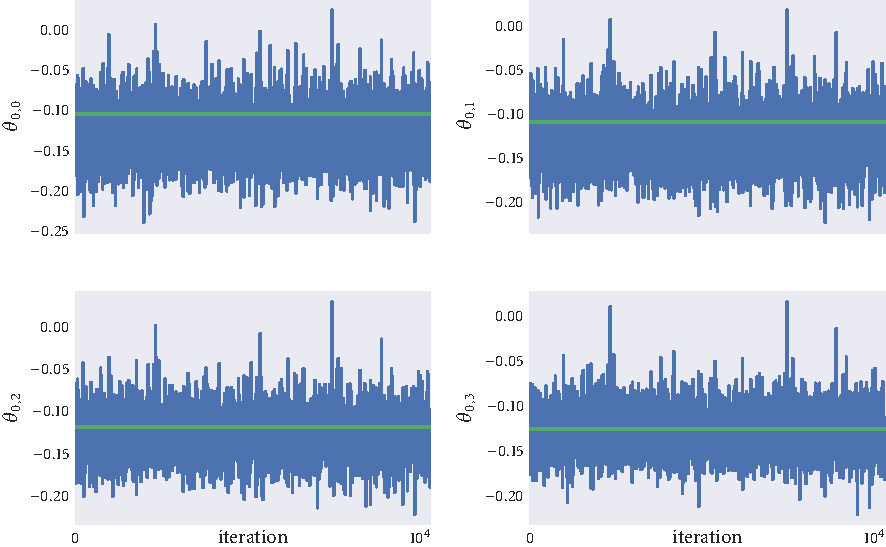
\includegraphics{beg/dir_trace.pdf}
  \caption{Chains targeting directions of motion missing at the beginning of a
    simulation. Each trajectory was simulated for 100,000 iterations. To
    decrease the autocorrelation between samples and reduce memory overhead
    the output was thinned by a factor of 10. The true values of the
    missing directions are shown by the horizontal green lines. The true
    values are captured within our posterior densities.}
  \label{fig:beg_dir_trace}
\end{figure}

\cref{fig:beg_x_trace} shows chains targeting the missing $x$ co-ordinates of
agent 6 over the first four frames. The chains targeting the $x$ co-ordinates
are related to the chains targeting the missing directions through
\cref{eq:propose_beg_pos}. \cref{fig:beg_x_trace} gives further evidence that
our chains have converged, and that the further back in time we extrapolate the
less certain we become about an agent's whereabouts.

\begin{figure}[tbp]
  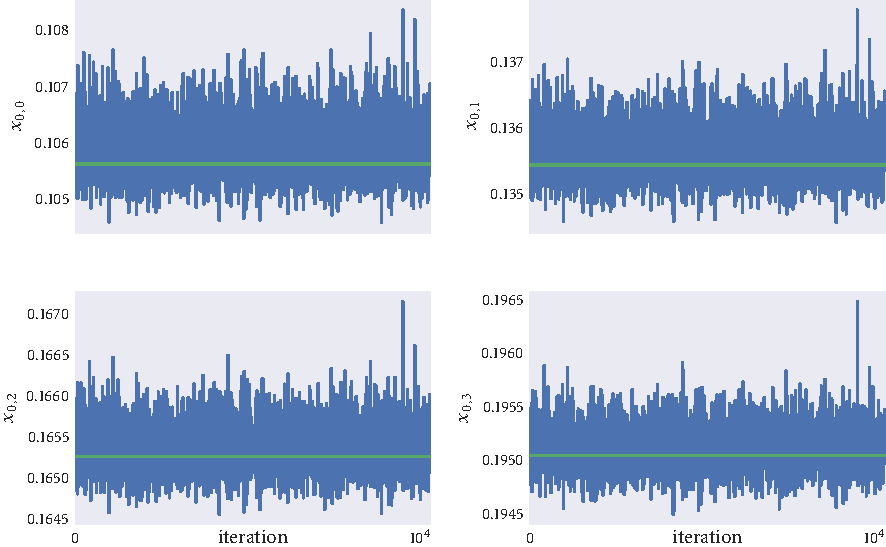
\includegraphics{beg/x_trace.pdf}
  \caption{Trajectories of the $x$ co-ordinates of agents corresponding to the
  directions of motion seen in \cref{fig:beg_dir_trace}. Sampled directions of
  motion are related to sampled co-ordinates through \cref{eq:propose_beg_pos}.
  The true values of the missing co-ordinates are overlain in green.}
  \label{fig:beg_x_trace}
\end{figure}

\begin{figure}[tbp]
  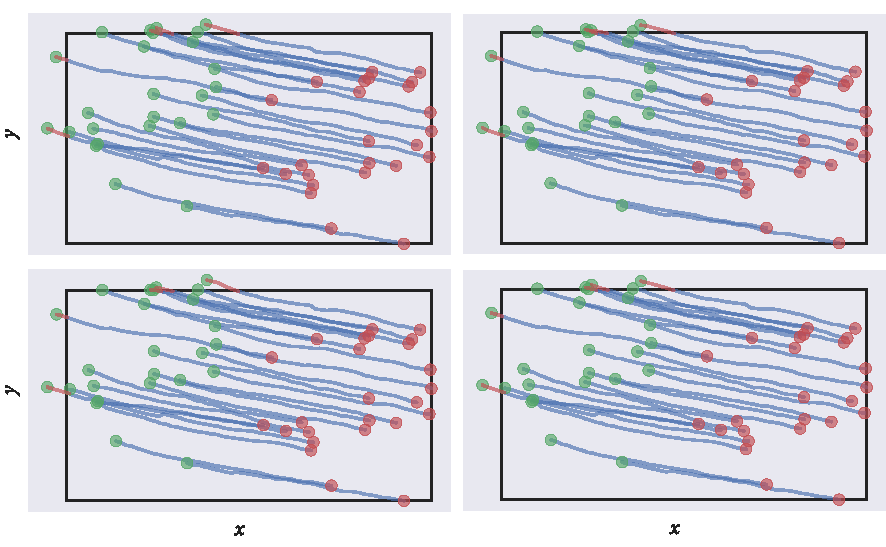
\includegraphics{beg/paths.pdf}
  \caption{Visualising completed paths at four randomly chosen iterations
  of our inference scheme. The plots show plausible trajectories were
  constructed by our scheme.}
  \label{fig:beg_paths}
\end{figure}

As with the hierarchical models considered in \cref{sec:hier_mod_studies}, we
now have a posterior distribution with a large number of dimensions, and so
assessing and presenting every marginal posterior density becomes impractical.
Instead, we summarise the output of our chains targeting the missing
observations in \cref{fig:beg_summary}. Each panel of \cref{fig:beg_summary}
shows box and whisker plots summarising our posterior samples. The yellow
markers show the posterior median, the inner-extent of the whiskers show the
upper and lower quartiles, and the outer-extent of the whiskers show the
posterior median $\pm1.5\times\text{IQR}$.

\begin{figure}[tbp]
  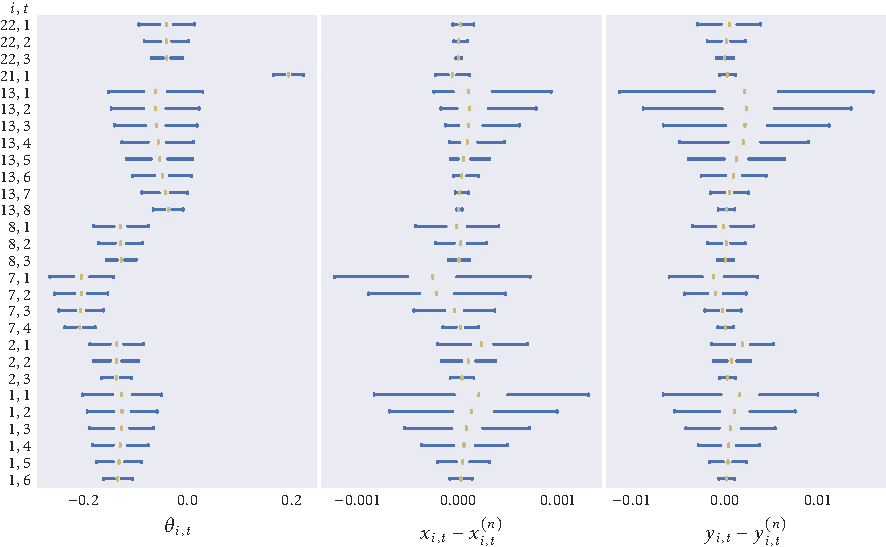
\includegraphics{beg/summary.pdf}
  \caption{Summarising the posterior samples targeting the missing directions
  of motion (left), $x$ co-ordinates (centre), and $y$ co-ordinates (right).
  True values are shown by the green markers, and posterior medians are shown
  by the yellow markers. The box and whisker plots show the upper and lower
  quartiles as well as the median $\pm1.5\times\text{IQR}$. Realisations of the
  missing positions are subtracted from the corresponding true values to make
  comparison easier.}
  \label{fig:beg_summary}
\end{figure}

The left-most panel of \cref{fig:beg_summary} summarises the posterior
densities representing our beliefs about the missing directions of motion. The
green markers represent true values. See that as we extrapolate further back in
time our posterior variance increases, as we would expect. The $x$ and $y$
co-ordinates corresponding to these directions are shown in the central and
right-most panels. As the between-agent variance in positions is much greater
than our posterior variance, to compare all the inferred positions in one plot
we first subtract the realised samples from the true values. This results in
box and whisker plots centered approximately around zero (shown by the green
markers): indicating that our posterior densities accurately captured the true
values. Again, we see that our posterior variance about the inferred positions
increases the further back in time we extrapolate.

We have shown that we can capture missing observations by implementing a
Metropolis--Hastings sampler. Now that we have this, we wish to inspect how
having missing observations has influenced our parameter uncertainty. We also
wish to investigate how our approach to missing data compares to the more
naive approach of discarding frames which don't capture every individual. To
make this comparison we re-perform parameter inference on the simulated data,
in the first instance increasing our field of vision to capture all
agents, and in the second instance discarding frames where any individual is
missing. We expect that the posterior variance about the model parameters with
the missingness accounted for should be greater than or equal to the posterior
variance had there been no missingness. Similarly, had we discarded the frames
with missingness, we would expect a posterior variance greater than or equal to
the posterior variance with the missingness integrated over. 

\cref{fig:beg_compare} compares posterior densities of the model parameters
under three different regimes: the flocking event without any missingness
(blue), the event with the missingness integrated out (red), and the event with
the missingness discarded (purple). From this plot we see that integrating over
the missing observations provides very similar posterior densities to if we had
observed all the data. We see that our approach to handling missingness gives
smaller posterior variance than the naive approach of discarding observations,
indicating the efficacy of our approach. As the computational demand of the
problem increases as more data goes missing, effort should still be made by the
scientist to minimise the total amount of missingness incurred during data
collection.

\begin{figure}[tbp]
  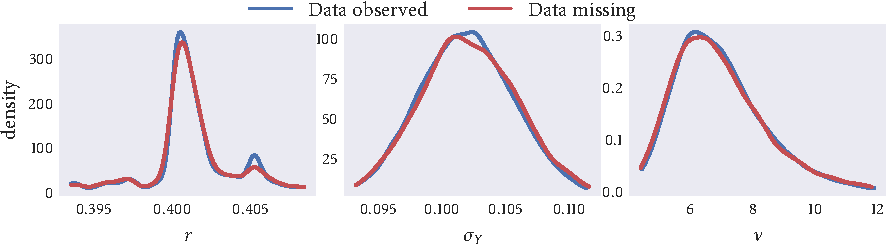
\includegraphics{beg/compare_params.pdf}
  \caption{Comparing posterior densities about the Vicsek model parameters had
    all the data been observed (blue); with the missingness integrated out
    (red), and when discarding frames which any individual is missing from
    (purple). The posterior densities are shown by kernel density estimates
    of the posterior samples.}
  \label{fig:beg_compare}
\end{figure}

\subsection{Missing in the end of a sequence}
\label{ssec:end_missing}

We say that data is missing at the end of a flocking event if some individuals
leave the frame of vision \emph{before} the recording event was completed. When
we consider this case we assume that agents which leave the frame do not later
re-enter it. We imitate this situation by simulating the movements of 25
individuals over 40 frames, according to the specifications of the Vicsek
model (here with parameters $r=0.45$, $\sigma_Y=0.07$ and $\nu=7$), and
overlaying a fixed field of vision. The resulting data is visualised in
\cref{fig:end_data}.

\begin{figure}[tbp]
  \captionsetup[subfigure]{oneside,
                           margin={0.7cm,0cm}}
  \begin{subfigure}[b]{0.5\textwidth}
    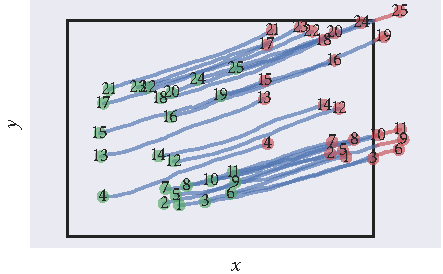
\includegraphics{end/data.pdf}
    \caption{}
    \label{subfig:end_data}
  \end{subfigure}%
  \begin{subfigure}[b]{0.5\textwidth}
    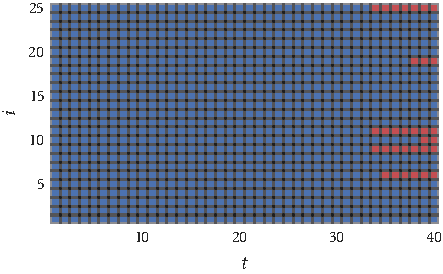
\includegraphics{end/missing_array.pdf}
    \caption{}
    \label{subfig:end_missing}
  \end{subfigure}
  \caption{Individuals missing at the end of a sequence.
  \subref{subfig:end_data} Twenty-five agents are simulated for forty frames
  according to the rules of the Vicsek model. Agents travel from the positions
  denoted by the green markers to those denoted by the red markers. The ID of
  each agent is shown at its start and end point. A fixed field of vision is
  emulated by the rectangle overlain in black. Any movements which occur
  outside this area are classified as missing; shown by trajectories
  transitioning from blue to red.
  \subref{subfig:end_missing} A representation of which data points of our
  simulation were observed and which were classified as missing. A blue tile at
  location $(t, i)$ indicates that agent $i$ was within our field of vision at
  time $t$. Conversely, a red tile at location $(t, i)$ indicates that agent
  $i$ was outside our field of vision---that is, missing---at time $t$.}
  \label{fig:end_data}
\end{figure}

To fit one of our models to this data we must be able to evaluate the
likelihood as specified in \cref{eq:likelihood}. This likelihood involves a
product over $i=1,\ldots,N$ and $t=1,\ldots,T$, and so we must have data to
represent these observations. As some agents are out of frame at the end of the
sequence, we do not have all the observations necessary to evaluate the
likelihood.

We can propose trajectories for the missing agents by forward simulating the
model from each agent's last observed position
(\cref{eq:students_update,eq:positional_update}). Doing so we write down the
full conditional distribution for missing directions at the end of a sequence
as:
\begin{equation}
  \theta_{i,t+1}^\star \given \angmean{\theta}_{i,t}, \nu, \sigma_Y \sim
  t_{\nu}(\angmean{\theta}_{i,t}, \sigma_Y)
\end{equation}
Realising paths missing at the end of a sequence is now achieved with a Gibbs
step (\cref{alg:gibbs}). With this there is no accept / reject step for the
sampled trajectories, and so new missing paths are evaluated at every iteration
of our sampler. As the sampled trajectories represent missing observations, any
samples that are generated within our field of vision are discarded and new
trajectories are sampled instead. This Gibbs step is embedded within a
Metropolis--Hastings sampler which works to infer the model parameters of the
Vicsek model.

\cref{fig:end_dir_trace} shows the chains targeting the missing directions of
motion of agent $i=6$. These trajectories show evidence of convergence and are
seen to capture the true values of the missing data (green). These directions
are related to the $y$-component of the missing positions (shown in
\cref{fig:end_y_trace}) via \cref{eq:positional_update}, and again capture the
true values of the missing data. \cref{fig:end_paths} goes to demonstrate that
the paths generated by our scheme are plausible: visualising four randomly
chosen flock configurations considered by our sampler.

In \cref{fig:end_dir_trace,fig:end_y_trace} we only inspect a small amount of
the total missingness targeted by our inference. \cref{fig:end_summary}
summarises the posterior densities about all the missing observations of our
simulated data. We see that in all cases the true values (green) are captured
within our posterior densities (blue). From the central and rightmost panels of
\cref{fig:end_summary} we see that posterior variance (uncertainty) increases
the further into the future we extrapolate.

\begin{figure}[tbp]
  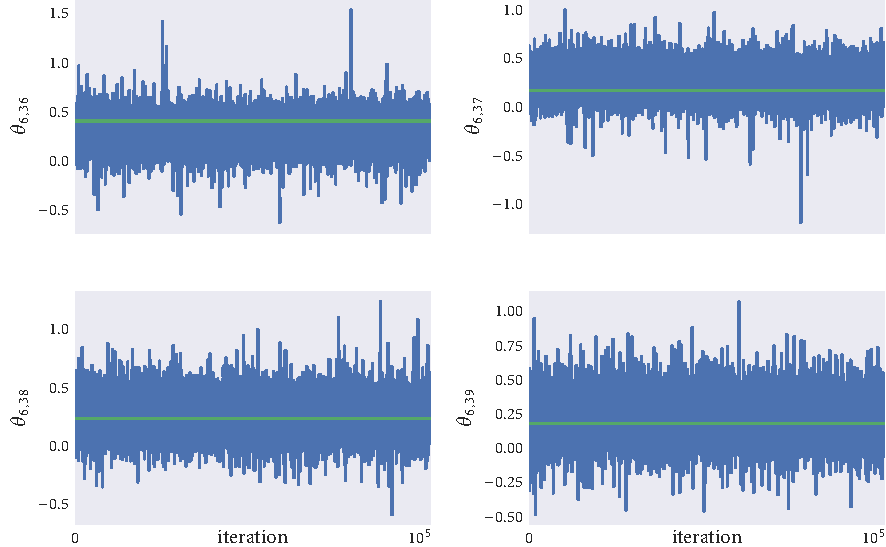
\includegraphics{end/dir_trace.pdf}
  \caption{Trace plots targeting directions of motion missing at the end of the
    simulated flocking event. The chains give strong evidence of convergence and
    show that the true values of the missing directions (green) are captured within
    the posterior densities.}
  \label{fig:end_dir_trace}
\end{figure}
\begin{figure}[tbp]
  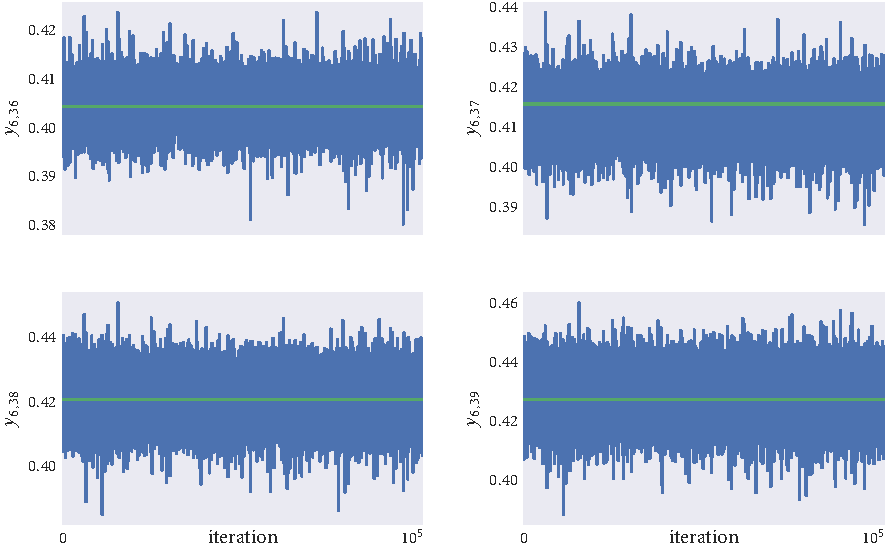
\includegraphics{end/y_trace.pdf}
  \caption{Trajectories targeting the $y$-component of the missing positions of
    agent $i=6$. The chains show evidence of convergence: oscillating around
    a fixed point with constant variance. The true values (green) are
    captured within the oscillations of the chains.}
  \label{fig:end_y_trace}
\end{figure}
\begin{figure}[tbp]
  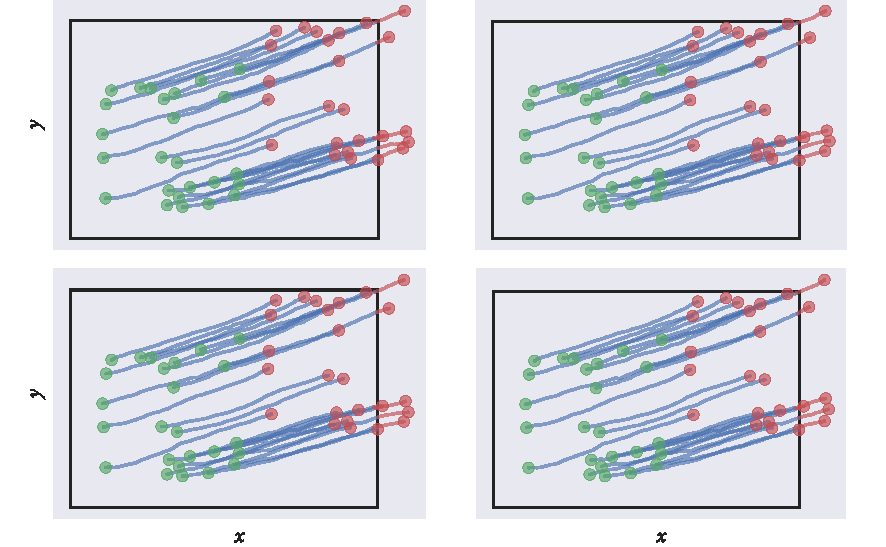
\includegraphics{end/paths.pdf}
  \caption{Visualising, at four randomly chosen iterations, missing
  trajectories that were completed by our inference scheme. The sampled paths
  look plausible.}
  \label{fig:end_paths}
\end{figure}
\begin{figure}[tbp]
  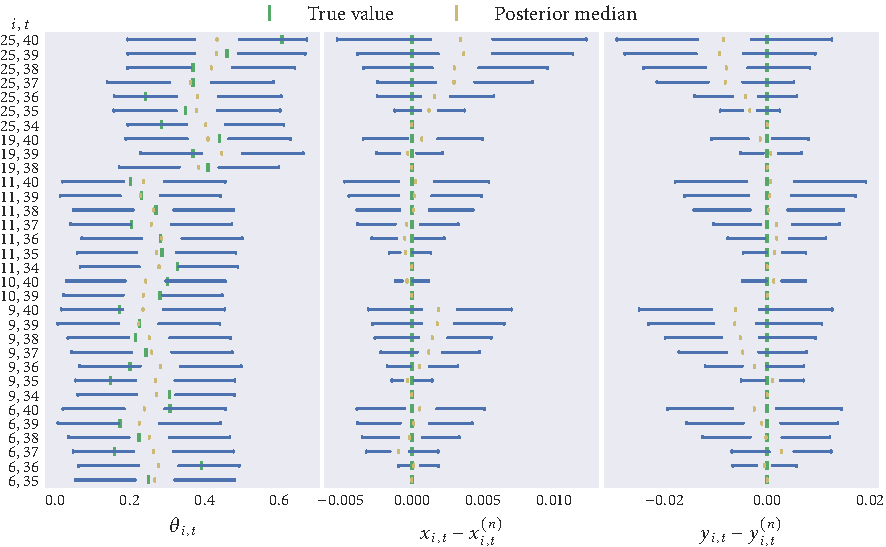
\includegraphics{end/summary.pdf}
  \caption{Summarising the posterior densities of the missing directions (left
  panel), $x$ co-ordinates (central panel), and $y$ co-ordinates (right
  panel). For comparative ease the samples of the missing positions are
  subtracted from the true missing positions. The true values being
  targeted are shown by the green markers, and all lie within the box and
  whisker plots representing our posterior densities. As we extrapolate further
  into the future we see that our posterior variance increases, as our
  uncertainty about the values of the missing observations increase.}
  \label{fig:end_summary}
\end{figure}

\cref{fig:end_summary} shows that our approach to missingness is able to
capture data missing at the end of a recording event. We now wish to inspect
how this approach has effected our posterior densities. To do so we perform
parameter inference on the simulated data as if all the data had been contained
within our field of vision. In addition to this we perform the same inference
but discarding all the frames in which any agent was out of view. The model
parameters inferred under these three scenarios are compared in
\cref{fig:end_compare}. We see that integrating out the missingness reveals
results similar to as if we had observed all the data, and that the naive
approach of discarding missingness resulted in a larger posterior variance.

The Gibbs sampler explores the sample space more efficiently than the
Metropolis--Hastings algorithm, an artefact of Gibbs' lack of an accept / reject
step. As a result we can handle data missing at the end of a sequence with
less computational expense than data missing at the beginning of a sequence.
We conclude that although all effort should be made by the scientist to avoid
recording sequences with any missing observations, where possible care should
be taken to bias the occurrence of data missing at the end of a sequence over
data missing at the beginning of a sequence.

\begin{figure}
  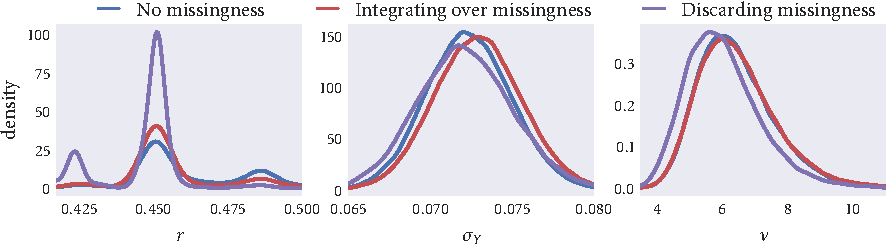
\includegraphics{end/compare_params.pdf}
  \caption{Kernel density estimates of the model parameters inferred from
  simulated data. The blue kernels represent posterior densities when the
  field of vision was widened to include all movements; the red kernels
  show posterior densities when the missingness was integrated out, and the
  purple kernels represent the posterior samples when all the frames
  containing missing data were discarded.}
  \label{fig:end_compare}
\end{figure}

\subsection{Missing in the beginning and end of a sequence}

Having demonstrated that we can handle sequences with observations missing at
the \emph{beginning} of an event and sequences with observations missing at the
\emph{end} of an event, we now seek to verify that we can handle sequences with
data missing at the beginning \emph{and} end. Having considered these two cases
separately we now consider them jointly. 

To handle sequences with data missing at the beginning and end, it is
sufficient to use the Gibbs step as outlined in \cref{ssec:end_missing} to
sample paths missing at the end of the sequence, and the Metropolis--Hastings
algorithm as in \cref{ssec:beg_missing} to propose paths missing at the
beginning of the sequence.

The data simulated for this study are shown in \cref{fig:both_data}. See that
the simulated data shows data points missing at the beginning \emph{and} end of
the event. This is again seen in \ref{subfig:both_missing}, which illustrates
which data points were observed and which classified as missing.

\begin{figure}[tbp]
  \captionsetup[subfigure]{oneside,
                           margin={0.7cm,0cm}}
  \begin{subfigure}[b]{0.5\textwidth}
    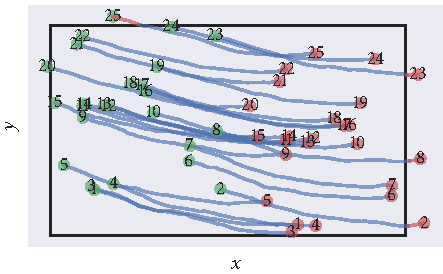
\includegraphics{both/data.pdf}
    \caption{}
    \label{subfig:both_data}
  \end{subfigure}%
  \begin{subfigure}[b]{0.5\textwidth}
    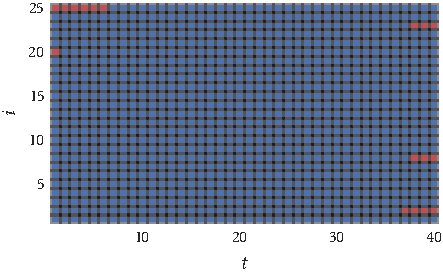
\includegraphics{both/missing_array.pdf}
    \caption{}
    \label{subfig:both_missing}
  \end{subfigure}
  \caption{Simulated data with observations missing at the beginning and end of
    the sequence. \subref{subfig:both_data} Showing the trajectories of the
    simulated agents. The rectangle overlain in black shows the simulated
    field of vision. As agents move from the green markers to the red markers
    we see that there are agents missing at the beginning and end of the
    sequence. \subref{subfig:both_missing} Schematic illustrating which data
    points were observed and which were classified as missing; a blue marker
    represents an observed data point, and a red marker represents a missing data
    point.}
  \label{fig:both_data}
\end{figure}

We fit the Vicsek model to this simulated data using our implementation of the
Metropolis--Hastings algorithm. Parameter inference is performed on (\emph{i})
data with no missingness, (\emph{ii}) data with missingness integrated out and
(\emph{iii}) data with missingness discarded. The posterior densities realised
under these three regimes are compared in \cref{fig:both_compare}. From this
figure we see that integrating over the missingness resulted in posterior
densities most similar to the densities with all the data observed.

\begin{figure}[tbp]
  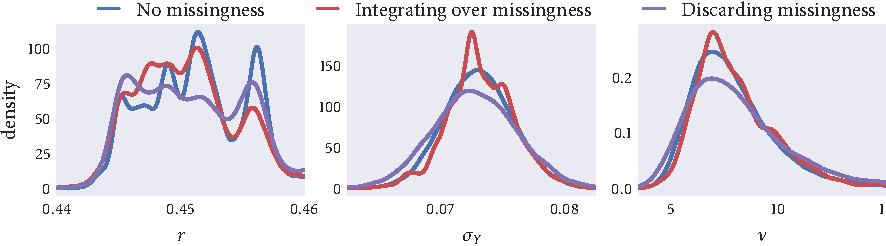
\includegraphics{both/compare_params.pdf}
  \caption{Comparing posterior densities about the parameters of the Vicsek
  model with and without missingness. The blue kernels show the posterior
  densities as if all the data was observed. The red kernels show the
  posteriors when the missing observations were integrated out. Finally, the
  purple kernels shows the posterior beliefs had the missing observations been
  discarded.}
  \label{fig:both_compare}
\end{figure}


\section{Case Study II: foraging scoters}
\label{sec:scoters}

In \cref{sec:missing_types} we discussed how the use of fixed-location recording
equipment during data acquisition can result in individuals moving out-of-frame
\emph{during} recording. Such movements are then missing from the recorded
flocking event. As out-of-frame movement may still be influencing the behaviour
of the observed flock, this movement must be accounted for during model
fitting.

In this section we consider a \emph{real} flocking event with missing
observations. As foreshadowed in the previous sections, the missing
observations of this dataset will be realised as a consequence of employing
fixed-location recording equipment.

The dataset considered  describes the movements of a large number of surf
scoters, a migratory sea bird, which gather in groups to forage. The captured
flocking events take place on the surface of a lake, and so movement is
effectively restricted to a two-dimensional plane. This dataset was provided
courtesy of work performed by \textcite{lukeman09,lukeman10}. At the time of
their publication the captured events represented a tenfold increase in the
number of individuals which could be reliably linked \emph{between} frames.

Unfortunately, owing to the fixed-location cameras used to record these
flocking events, there were often scoters out of view in the recorded frames.
\cref{fig:lukeman_extraction} illustrates the steps performed to extract the
positions of individuals from raw footage; this figure also shows how the flock
occupied an area larger than that which the camera captured---resulting in
missing observations. As earlier, the missing data points can be partitioned
into observations missing at the \emph{beginning} of the recording event, and
observations missing at the \emph{end} of the recording event.

\subsection{Scoter data}

\textcite{lukeman10} recorded a number of flocking events from an aerial
vantage point: an elevated promenade at the side of a large lake. From this
position the authors were able to direct a camera toward an inlet where
overwintering scoters had been observed foraging. Knowing the height of this
camera above the water, and the angle of its approach with the horizontal, the
authors were able to transform the captured camera data back to ``real-world''
co-ordinates.

However, to reliably transform back from camera co-ordinates to real-world
co-ordinates, the height of the camera above the lake and its angle with the
horizontal had to be fixed. With the camera fixed in position, the authors then
waited for flocking events to occur. Recording began when individuals entered
the camera's field of vision, and ended when all the individuals left the
frame, or the flock became stationary. Each recording event captured the
movements of around 170 scoters, with each event consisting of approximately
30 frames. However, of the recorded events between $16\%$ and $64\%$ of each
flock's movements took place out-of-frame.

\textcite{lukeman10} discounted the influence of individuals out-of-frame, and
instead focused on reproducing radial and angular neighbour densities of
\emph{internal} group members (edge individuals were also discarded). This
approach, although representing a significant step forward in the literature,
came with its drawbacks. Most significantly, focusing the fitting on
reproducing radial and angular neighbour distributions removed the
\emph{dynamic} component to the data which the authors worked so hard to
achieve. Additionally, the authors determined the size of the agents'
interaction radius by visual inspection of nearest-neighbour densities; the
interaction radius used in their model being chosen \emph{before} the fitting
process began.

In this chapter we take a more holistic approach to model fitting; making sure
to account for \emph{all} individuals---both observed and missing, as well as
internal and boundary individuals---and focusing the fitting on reproducing
the \emph{movements} of the flock, rather than some epiphenomena of their
movements. Significant computation is necessary to account for the large amount
of data missing from the recorded flocking events.

\subsection{Model fitting}

As the computational demands of missing data problems increase as the amount of
missingness increases, we focus on the flocking event within the Lukeman dataset
which displays the \emph{least} amount of missingness. For the events captured
by \textcite{lukeman10} this is represented by a sequence of 199 scoters
moving over 23 frames. Of the $199\times23=4,577$ data points represented by
this event, 680 ($\approx16\%)$ occur outside the visual field of the camera.
This flock is visualised in \cref{fig:scoter_traj}. From this figure we see
that the flock was strongly polarised throughout the recording event; with this
observation we consider an alignment-based model a plausible candidate model
for fitting.

\begin{figure}[tb]
  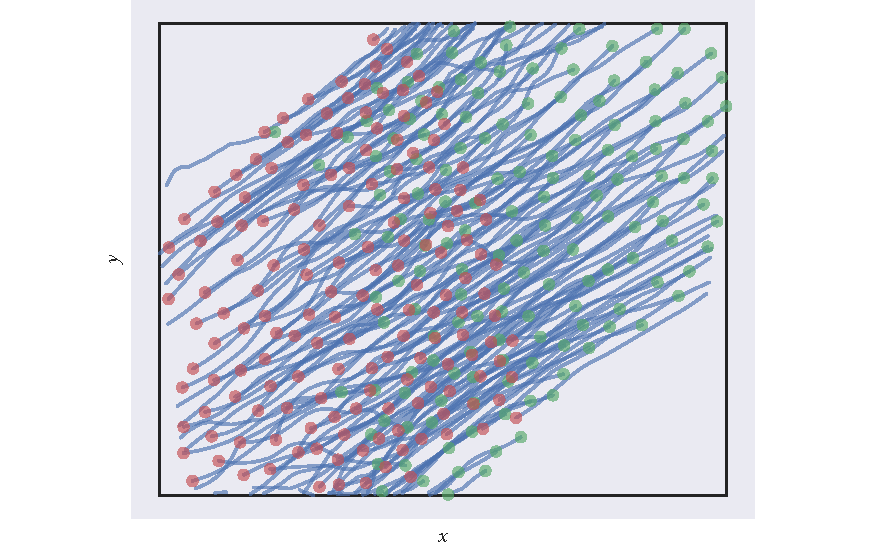
\includegraphics{data_00_traj.pdf}
  \caption{A visualisation of the trajectories of foraging surf scoters in an
    analysed sequence. In total, the sequence represents the movements of
    199 scoters over 23 frames (4,577 data points). The scoters move
    along the blue trajectories, starting from the positions denoted by the
    green markers and finishing at the positions shown by the red markers. The
    black frame containing the trajectories represents an approximation of the
    fixed field of vision of the recording equipment.}
  \label{fig:scoter_traj}
\end{figure}

\cref{fig:scoter_missing} gives a visual representation of which data points
were observed, and which data points were missing. In this visualisation blue
markers represent observed data and red markers represent missing data. From
\cref{fig:scoter_missing} we see that in \emph{every frame} there is \emph{at
least one} missing scoter. As such, if we were to discard all the frames with
as least one missing scoter (as in the naive approach), we would discard the
\emph{entire} flocking event. Therefore, to evaluate the likelihood of observing
this flock we have no choice but to account for the missing observations.

The simulated flocks considered in \cref{ssec:beg_missing,ssec:end_missing} had
between 10 and 20 missing observations per sequence. With 680 data points
missing from the scoter sequence with the \emph{least} amount of missingness,
this problem represents a considerable increase in complexity. With this amount
of missingness, long and expensive simulations were necessary to realise a
satisfactory number of samples from the posterior.

% XXX: Label axis explicitly: Individual (i)
% Would missing be nicer as white? Not sure
\begin{figure}[tb]
  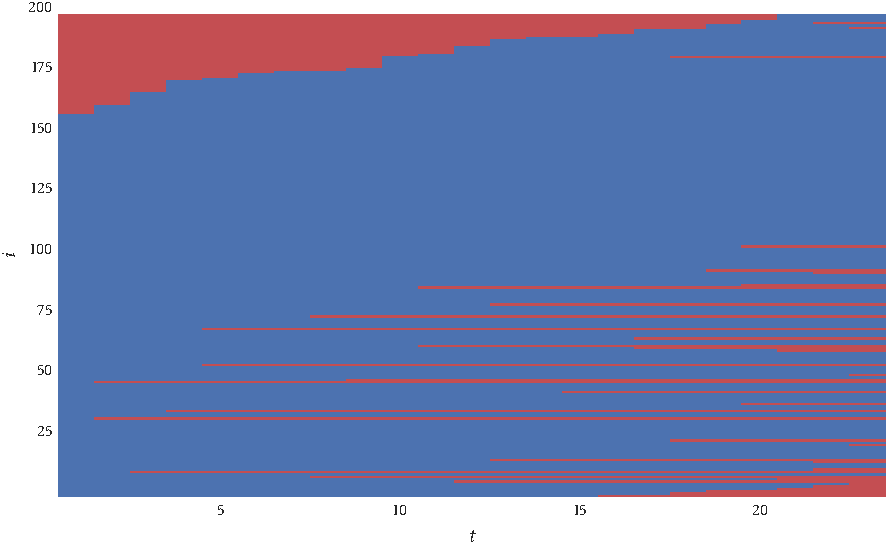
\includegraphics{data_00_missing.pdf}
  \caption{A representation of the missing and observed data points of the
    foraging event illustrated in \cref{fig:scoter_traj}. The $x$-axis
    represents the frame of the sequence, and the $y$-axis corresponds to
    tracked individuals. A blue tile at location $(t, i)$ tells us that scoter
    $i$ was observed in frame $t$. A red tile at location $(t, i)$ indicates
    that scoter $i$ was missing at time $t$.}
  \label{fig:scoter_missing}
\end{figure}

%XXX: Not read chap 7 yet, but do you mention why not Stan?
We fit a variation of the Vicsek model to this dataset where each agent
interacts with neighbours within distance $r$ (\cref{eq:vicsek_interaction}),
and experiences noise sampled from a generalised Student's $t$ distribution
with $\nu$ degrees of freedom and scale $\sigma_Y$ (\cref{eq:students_update}).
A random walk Metropolis--Hastings algorithm was implemented to infer the
parameters of this model. In a similar manner, a random walk
Metropolis--Hastings algorithm, with proposal scheme as outlined in
\cref{ssec:beg_missing}, was used to infer the observations missing at the
beginning of the sequence. Finally, using a Gibbs step allowed observations
missing at the end of the sequence to be sampled. This sampler was implemented
for $10^8$ iterations. To reduce the memory overhead of this sampler, the
recorded samples were thinned by a factor of 1000; meaning that all but every
1000th iteration of the sampler was discarded, producing a total of $10^8 /
10^3 = 10^5$ samples.

Previously we used summary plots---such as those in
\cref{fig:beg_summary,fig:end_summary}---to help visualise high-dimensional
posterior distributions. However, with almost 700 dimensions, this posterior
has too many dimensions for even these summary plots. In such a situation it
can be informative to graphically assess the trace of the log-likelihood. If we
can observe that the log-likelihood has converged, we have strong evidence that
the sampler has converged. In \cref{fig:log_ll} we see a trace and histogram
plot of evaluations of the log-likelihood. From this plot we see evidence of
convergence, as the log-likelihood oscillates regularly around some fixed
location.

% XXX: Note sure if it's worth sticking a loess smoother through
% the LL, to show it's stable?
\begin{figure}[tb]
  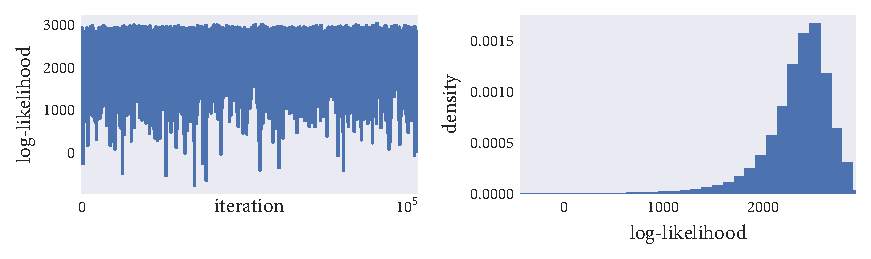
\includegraphics{log_likelihood.pdf}
  \caption{Trace and histogram plots of the log-likelihood, as computed at
    every iteration of the inference scheme. As it can be difficult to assess
    the convergence of all the parameters for high-dimensional problems, as
    we have here, it can instead be informative to assess the convergence of
    the log-likelihood. If we see that the value of the log-likelihood has
    converged, then we have evidence that the chains targeting the corresponding
    parameters also converged.}
    \label{fig:log_ll}
\end{figure}

The parameters of the Vicsek model inferred in this fitting are shown in
\cref{fig:lukeman_params}. The tendency of the interaction radius $r$ towards
zero suggests that there is no direct alignment interaction between individuals
of this flock. The flock's highly polarised structure must then be the result
of behaviours unaccounted for by our model: such as attraction or repulsion
interactions. With no effective interaction term, all observed directional
changes must be accounted for by the inferred noise parameters, as in the Null
model (\cref{sec:null_model}). The inferred degrees of freedom and noise-scale
parameters represent a diffuse noise distribution, reflecting their need to
capture all directional changes.

\begin{figure}[tb]
  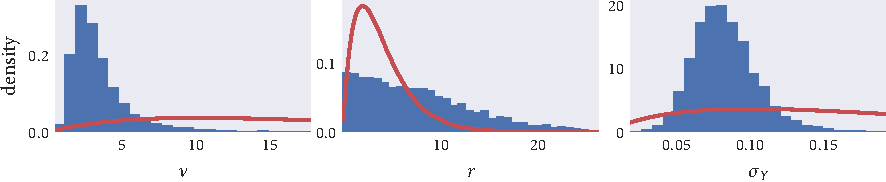
\includegraphics{params_hist.pdf}
  \caption{Samples drawn from the posterior distribution realised in fitting a
    sequence of the Lukeman data to a variation of the Vicsek model. The
    posterior distribution of $r$ is non-normal, and tends towards zero,
    representing evidence that there is no explicit alignment interaction
    between individuals.}
  \label{fig:lukeman_params}
\end{figure}

In \cref{fig:dir_hist} we see histogram plots of samples realised from the
posterior: here representing four directions missing at the end of the
sequence. We see that the uncertainty in the possible directions of motion of
the missing agent is large. This large posterior variance is a result of the
large amounts of missingness. As no effective interaction term was realised, a
diffuse noise structure was inferred to account for the observed directional
changes. This diffuse noise structure further contributes to the large
posterior variance inferred for the missing directions.

Although our model has been unable to capture the interactions between
individuals present in this flock, it is only by handling the missing data that
we have been able to fit this model and make this realisation.

\begin{figure}[tb]
  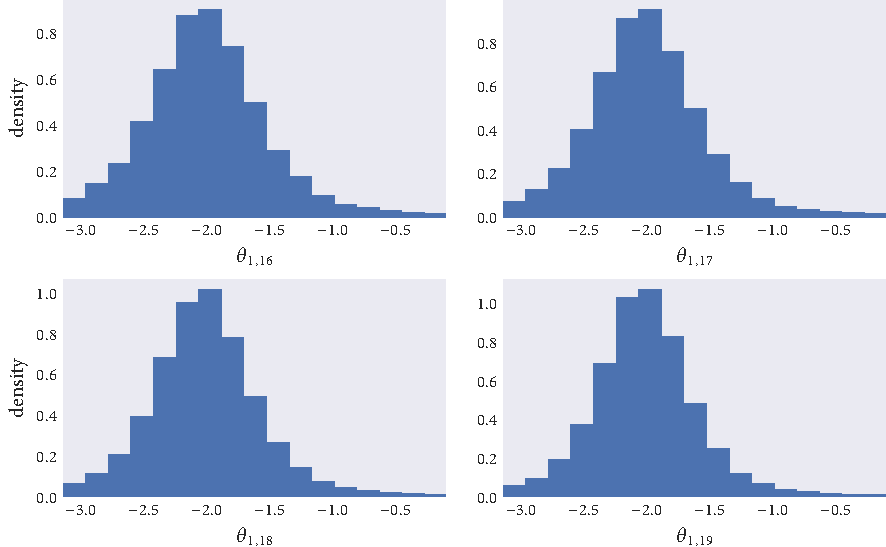
\includegraphics{dir_hist.pdf}
  \caption{Histogram plots of posterior draws of 4 missing directions (out of
    a total of 680 missing data points). The posterior draws visualised
    correspond to data missing at the end of the sequence. We see large amounts
    of uncertainty in these posterior densities, reflecting the large amount of
    missingness represented by this sequence.}
  \label{fig:dir_hist}
\end{figure}

\section*{Conclusions}

In this chapter we considered the experimental set-ups required to record
flocking events in the wild. We saw missing data arises naturally as a
consequence of recording data with fixed-location cameras. However, as
individuals which move out of frame may still be influencing the movements
of the observed flock, they cannot simply be ignored.

A naive approach to this missing data problem would be to discard \emph{all}
the frames in which \emph{any single} agent moves out of frame. Although this
approach allows us to evaluate the likelihood of the flock---and hence perform
our desired fitting---it has the potential to drastically reduce the amount of
data available for analysis.

We outlined an alternative approach in which all possible out-of-frame
movements are integrated over. For this approach we first partition missing
data points into observations missing at the \emph{beginning} of a recording
event and observations missing at the \emph{end} of a recording event. With this
we outlined inference schemes which could infer data missing under these two
regimes.

Simulation studies were performed in which an artificial fixed field of vision
was overlain on the data. We demonstrated that our inference schemes were able
to capture the true values of the missing observations. We discussed how
increasing the amount of missing data increases the complexity, and hence
computational demand, of the problem. Although all care should be taken to
avoid recording events with missing observations, we advised that as data
missing at the end of a sequence could be handled at less computational expense
than data missing in the beginning, emphasis should be put on avoiding
observations going missing at the beginning of a sequence.

To consider the efficacy of our approach to missing data we compared posterior
densities generated when integrating over the missingness, to posterior
densities on the same dataset without missingness, and to posterior densities
realised with the missingness discarded (the naive approach). We found
that our approach to missingness generated posterior densities closer to the
``observed-all'' densities than the naive approach was able to. 

The developed methodology was then applied to a flocking event in which at
least one individual was out of view during every frame of the recording. Of
the 4,577 data points in the analysed sequence, 680 ($\approx16\%$) of the
observations were missing. To evaluate the likelihood of this data we had to be
able to account for the position and direction of every individual in the
analysed frames. As at least one individual is missing in every frame,
discarding frames containing missingness is not a viable solution.

The large amount of missing data in the analysed sequence resulted in a
high-dimensional posterior distribution, and hence a computationally intensive
inference problem. Long simulations were necessary to allow the simulated
Markov chains to achieve convergence. Although the inference scheme converged,
our results showed evidence that there is no explicit alignment interaction
between individuals, suggesting the presence of interactions not accounted for
by our model. As our model couldn't capture these interactions, it instead
attempted to account for directional changes through noise alone, which in turn
resulted in large uncertainties about missing positions and directions of
motion. Despite our candidate model being unable to capture the interactions
between individuals, it was only by handling this missing data that we were
able to come to this realisation.
